
\documentclass[letterpaper,hide notes,xcolor={table,svgnames},pdftex]{beamer}
\def\showexamples{t}


%\usepackage[svgnames]{xcolor}

%% Demo talk
%\documentclass[letterpaper,notes=show]{beamer}

\usecolortheme{crane}
\setbeamertemplate{navigation symbols}{}

\usetheme{MyPittsburgh}
%\usetheme{Frankfurt}

%\usepackage{tipa}

\usepackage{hyperref}
\usepackage{graphicx,xspace}
\usepackage[normalem]{ulem}

\newcommand\SF[1]{$\bigstar$\footnote{SF: #1}}



\newcounter{tmpnumSlide}
\newcounter{tmpnumNote}

% old question code
%\newcommand\question[1]{{$\bigstar$ \small \onlySlide{2}{#1}}}
% \newcommand\nquestion[1]{\ifdefined \presentationonly \textcircled{?} \fi \note{\par{\Large \textbf{?}} #1}}
% \newcommand\nanswer[1]{\note{\par{\Large \textbf{A}} #1}}


 \newcommand\mnote[1]{%
   \addtocounter{tmpnumSlide}{1}
   \ifdefined\showcues {~\tiny\fbox{\arabic{tmpnumSlide}}}\fi
   \note{\setlength{\parskip}{1ex}\addtocounter{tmpnumNote}{1}\textbf{\Large \arabic{tmpnumNote}:} {#1\par}}}

\newcommand\mmnote[1]{\note{\setlength{\parskip}{1ex}#1\par}}

%\newcommand\mnote[2][]{\ifdefined\handoutwithnotes {~\tiny\fbox{#1}}\fi
% \note{\setlength{\parskip}{1ex}\textbf{\Large #1:} #2\par}}

%\newcommand\mnote[2][]{{\tiny\fbox{#1}} \note{\setlength{\parskip}{1ex}\textbf{\Large #1:} #2\par}}

\newcommand\mquestion[2]{{~\color{red}\fbox{?}}\note{\setlength{\parskip}{1ex}\par{\Large \textbf{?}} #1} \note{\setlength{\parskip}{1ex}\par{\Large \textbf{A}} #2\par}\ifdefined \presentationonly \pause \fi}

\newcommand\blackboard[1]{%
\ifdefined   \showblackboard
  {#1}
  \else {\begin{center} \fbox{\colorbox{blue!30}{%
         \begin{minipage}{.95\linewidth}%
           \hspace{\stretch{1}} Some space intentionally left blank; done at the blackboard.%
         \end{minipage}}}\end{center}}%
         \fi%
}



%\newcommand\q{\tikz \node[thick,color=black,shape=circle]{?};}
%\newcommand\q{\ifdefined \presentationonly \textcircled{?} \fi}

\usepackage{listings}
\lstset{%
  keywordstyle=\bfseries,
  aboveskip=15pt,
  belowskip=15pt,
  captionpos=b,
  identifierstyle=\ttfamily,
  escapeinside={(*@}{@*)},
  stringstyle=\ttfamiliy,
  frame=lines,
  numbers=left, basicstyle=\scriptsize, numberstyle=\tiny, stepnumber=0, numbersep=2pt}

\usepackage{siunitx}
\newcommand\sius[1]{\num[group-separator = {,}]{#1}\si{\micro\second}}
\newcommand\sims[1]{\num[group-separator = {,}]{#1}\si{\milli\second}}
\newcommand\sins[1]{\num[group-separator = {,}]{#1}\si{\nano\second}}
\sisetup{group-separator = {,}, group-digits = true}

%% -------------------- tikz --------------------
\usepackage{tikz}
\usetikzlibrary{positioning}
\usetikzlibrary{arrows,backgrounds,automata,decorations.shapes,decorations.pathmorphing,decorations.markings,decorations.text}

\tikzstyle{place}=[circle,draw=blue!50,fill=blue!20,thick, inner sep=0pt,minimum size=6mm]
\tikzstyle{transition}=[rectangle,draw=black!50,fill=black!20,thick, inner sep=0pt,minimum size=4mm]

\tikzstyle{block}=[rectangle,draw=black, thick, inner sep=5pt]
\tikzstyle{bullet}=[circle,draw=black, fill=black, thin, inner sep=2pt]

\tikzstyle{pre}=[<-,shorten <=1pt,>=stealth',semithick]
\tikzstyle{post}=[->,shorten >=1pt,>=stealth',semithick]
\tikzstyle{bi}=[<->,shorten >=1pt,shorten <=1pt, >=stealth',semithick]

\tikzstyle{mut}=[-,>=stealth',semithick]

\tikzstyle{treereset}=[dashed,->, shorten >=1pt,>=stealth',thin]

\usepackage{ifmtarg}
\usepackage{xifthen}
\makeatletter
% new counter to now which frame it is within the sequence
\newcounter{multiframecounter}
% initialize buffer for previously used frame title
\gdef\lastframetitle{\textit{undefined}}
% new environment for a multi-frame
\newenvironment{multiframe}[1][]{%
\ifthenelse{\isempty{#1}}{%
% if no frame title was set via optional parameter,
% only increase sequence counter by 1
\addtocounter{multiframecounter}{1}%
}{%
% new frame title has been provided, thus
% reset sequence counter to 1 and buffer frame title for later use
\setcounter{multiframecounter}{1}%
\gdef\lastframetitle{#1}%
}%
% start conventional frame environment and
% automatically set frame title followed by sequence counter
\begin{frame}%
\frametitle{\lastframetitle~{\normalfont(\arabic{multiframecounter})}}%
}{%
\end{frame}%
}
\makeatother

\makeatletter
\newdimen\tu@tmpa%
\newdimen\ydiffl%
\newdimen\xdiffl%
\newcommand\ydiff[2]{%
    \coordinate (tmpnamea) at (#1);%
    \coordinate (tmpnameb) at (#2);%
    \pgfextracty{\tu@tmpa}{\pgfpointanchor{tmpnamea}{center}}%
    \pgfextracty{\ydiffl}{\pgfpointanchor{tmpnameb}{center}}%
    \advance\ydiffl by -\tu@tmpa%
}
\newcommand\xdiff[2]{%
    \coordinate (tmpnamea) at (#1);%
    \coordinate (tmpnameb) at (#2);%
    \pgfextractx{\tu@tmpa}{\pgfpointanchor{tmpnamea}{center}}%
    \pgfextractx{\xdiffl}{\pgfpointanchor{tmpnameb}{center}}%
    \advance\xdiffl by -\tu@tmpa%
}
\makeatother
\newcommand{\copyrightbox}[3][r]{%
\begin{tikzpicture}%
\node[inner sep=0pt,minimum size=2em](ciimage){#2};
\usefont{OT1}{phv}{n}{n}\fontsize{4}{4}\selectfont
\ydiff{ciimage.south}{ciimage.north}
\xdiff{ciimage.west}{ciimage.east}
\ifthenelse{\equal{#1}{r}}{%
\node[inner sep=0pt,right=1ex of ciimage.south east,anchor=north west,rotate=90]%
{\raggedleft\color{black!50}\parbox{\the\ydiffl}{\raggedright{}#3}};%
}{%
\ifthenelse{\equal{#1}{l}}{%
\node[inner sep=0pt,right=1ex of ciimage.south west,anchor=south west,rotate=90]%
{\raggedleft\color{black!50}\parbox{\the\ydiffl}{\raggedright{}#3}};%
}{%
\node[inner sep=0pt,below=1ex of ciimage.south west,anchor=north west]%
{\raggedleft\color{black!50}\parbox{\the\xdiffl}{\raggedright{}#3}};%
}
}
\end{tikzpicture}
}


%% --------------------

%\usepackage[excludeor]{everyhook}
%\PushPreHook{par}{\setbox0=\lastbox\llap{MUH}}\box0}

%\vspace*{\stretch{1}

%\setbox0=\lastbox \llap{\textbullet\enskip}\box0}

\setlength{\parskip}{\fill}

\newcommand\noskips{\setlength{\parskip}{1ex}}
\newcommand\doskips{\setlength{\parskip}{\fill}}

\newcommand\xx{\par\vspace*{\stretch{1}}\par}
\newcommand\xxs{\par\vspace*{2ex}\par}
\newcommand\tuple[1]{\langle #1 \rangle}
\newcommand\code[1]{{\sf \footnotesize #1}}
\newcommand\ex[1]{\uline{Example:} \ifdefined \presentationonly \pause \fi
  \ifdefined\showexamples#1\xspace\else{\uline{\hspace*{2cm}}}\fi}

\newcommand\ceil[1]{\lceil #1 \rceil}


\AtBeginSection[]
{
   \begin{frame}
       \frametitle{Outline}
       \tableofcontents[currentsection]
   \end{frame}
}



\pgfdeclarelayer{edgelayer}
\pgfdeclarelayer{nodelayer}
\pgfsetlayers{edgelayer,nodelayer,main}

\tikzstyle{none}=[inner sep=0pt]
\tikzstyle{rn}=[circle,fill=Red,draw=Black,line width=0.8 pt]
\tikzstyle{gn}=[circle,fill=Lime,draw=Black,line width=0.8 pt]
\tikzstyle{yn}=[circle,fill=Yellow,draw=Black,line width=0.8 pt]
\tikzstyle{empty}=[circle,fill=White,draw=Black]
\tikzstyle{bw} = [rectangle, draw, fill=blue!20, 
    text width=4em, text centered, rounded corners, minimum height=2em]
    
    \newcommand{\CcNote}[1]{% longname
	This work is licensed under the \textit{Creative Commons #1 3.0 License}.%
}
\newcommand{\CcImageBy}[1]{%
	\includegraphics[scale=#1]{creative_commons/cc_by_30.pdf}%
}
\newcommand{\CcImageSa}[1]{%
	\includegraphics[scale=#1]{creative_commons/cc_sa_30.pdf}%
}
\newcommand{\CcImageNc}[1]{%
	\includegraphics[scale=#1]{creative_commons/cc_nc_30.pdf}%
}
\newcommand{\CcGroupBySa}[2]{% zoom, gap
	\CcImageBy{#1}\hspace*{#2}\CcImageNc{#1}\hspace*{#2}\CcImageSa{#1}%
}
\newcommand{\CcLongnameByNcSa}{Attribution-NonCommercial-ShareAlike}

\newenvironment{changemargin}[1]{% 
  \begin{list}{}{% 
    \setlength{\topsep}{0pt}% 
    \setlength{\leftmargin}{#1}% 
    \setlength{\rightmargin}{1em}
    \setlength{\listparindent}{\parindent}% 
    \setlength{\itemindent}{\parindent}% 
    \setlength{\parsep}{\parskip}% 
  }% 
  \item[]}{\end{list}} 



\usepackage{tikz-3dplot}

\title{Lecture 27 --- Verification \& Validation; Software Maintenance}

\author{Patrick Lam \& Jeff Zarnett \\ \small \texttt{p.lam@ece.uwaterloo.ca} \& \texttt{jzarnett@uwaterloo.ca}}
\institute{Department of Electrical and Computer Engineering \\
  University of Waterloo}
\date{\today}

\begin{document}

\begin{frame}
  \titlepage
\end{frame}

\part{Verification and Validation}
\frame{\partpage}

\begin{frame}
\frametitle{Verification vs validation}
\begin{changemargin}{1cm}

Two similar terms. Not the same.
\begin{itemize}
\item \structure{Verification}: ``Is the project being built correctly?''
\item \structure{Validation}: ``Will the project meet users' needs?''
\end{itemize}

Need both!\\[1em]

Projects can fail because:
\begin{itemize}
\item meet users' needs, but don't work right; or
\item bug-free but solve the wrong problem.
\end{itemize}~\\

{\Large A successful project must pass both verification and validation.}
\end{changemargin}
\end{frame}

\begin{frame}
\frametitle{More on Verification}
\begin{changemargin}{1cm}

\structure{Verification}:

\begin{itemize}
\item  assume a set of requirements; and
\item  establish that the product satisfies the
requirements.
\end{itemize}
The requirements might be wrong. Not our problem!\\[1em]

\structure{How to verify}: two options---
\begin{itemize}
\item testing (as seen previously);
\item static analysis\\ \quad (computers exhaustively check code/design).
\end{itemize}

\end{changemargin}

\begin{center}
``Building the thing right.''
\end{center}
\end{frame}

\begin{frame}
\frametitle{More on Validation}
\begin{changemargin}{1cm}

\structure{Validation}:

make sure that the requirements are the right ones.\\[1em]

(How does XP incorporate validation?)\\[1em]

Go beyond checking that code meets
specifications; \\
work with customer to ensure
specifications are correct. 


\end{changemargin}

\begin{center}
``Building the right thing.''
\end{center}


\begin{changemargin}{1cm}
One way to validate code: \emph{beta testing}.

\begin{itemize}
\item customers try the software and see if it's good.
\end{itemize}
\end{changemargin}

\end{frame}


\begin{frame}
\frametitle{Which first?}
\begin{changemargin}{1cm}

Verification, then validation.\\[1em]

Validating buggy software is frustrating.\\

Too much verification can be wasted work.
\end{changemargin}
\end{frame}


\begin{frame}
\frametitle{Independent V \& V}
\begin{changemargin}{1cm}

Sometimes V\&V processes are carried out by a different team.

This is known as \alert{Independent Verification and Validation}. 

Common in cases where there is extreme expense or risk to human life or health. 

NASA established IV\&V in 1993.

\end{changemargin}
\end{frame}

\begin{frame}
\frametitle{Regulatory Environment}
\begin{changemargin}{1cm}

Validation might be required given a regulatory environment. 

The US FDA requires software patches to be validated for networked medical devices. 

The device manufacturer bears responsibility for the safe and effective performance of the device.

FDA will review when a change or modification could significantly affect the safety or effectiveness of the device.

\end{changemargin}
\end{frame}

\part{Formal Methods}
\frame{\partpage}

\begin{frame}
\frametitle{About Formal Methods}
\begin{changemargin}{1cm}

Formal methods: techniques for \structure{verification}:\\
\qquad make sure that code/designs conform to a specification.\\[1em]

Some formal methods techniques:
\begin{itemize}
\item static analysis;
\item model checking.
\end{itemize}

\end{changemargin}
\end{frame}

\begin{frame}
\frametitle{Key Idea}
\begin{changemargin}{1cm}

To use formal methods, you need:
\begin{itemize}
\item a \structure{model} of the artifact in question; and,
\item a \structure{property} that you would like to verify.
\end{itemize}~\\

Often, the model is an abstract graph (ECE103!) representing
system behaviours.

The property is usually a temporal logic formula.\\[1em]

Verification exhaustively searches model for
violations.

\end{changemargin}
\end{frame}

\begin{frame}
\frametitle{Result of Verification}
\begin{changemargin}{1cm}

After the exhaustive search, either:
\begin{itemize}
\item the property definitely holds (on the model); or
\item you get a counterexample.
\end{itemize}

With cleverness, we can search huge state spaces ($10^{100}$ states).\\[1em]

Main insight: leveraging symmetries.
\end{changemargin}
\end{frame}

\begin{frame}
\frametitle{Case Study: Microsoft Static Driver Verifier}

\begin{center}
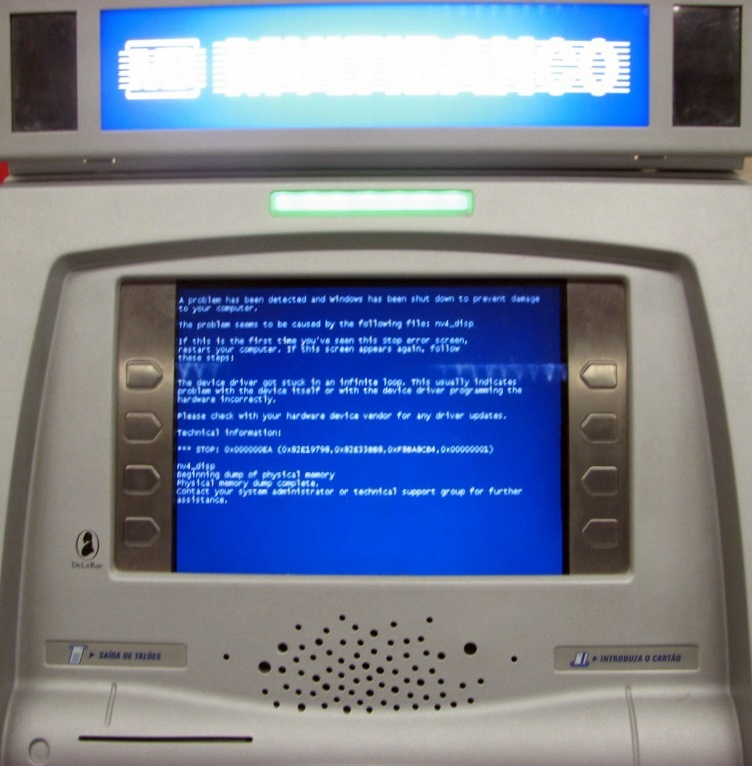
\includegraphics[width=\textwidth]{images/DeLaRue_ATM_Crash.jpg}
\end{center}

\end{frame}

\begin{frame}
\frametitle{Why does Windows crash?}

\begin{changemargin}{1cm}
Usually, not the Windows kernel---fairly bombproof now.\\

Instead: Windows drivers; run at same protection level as the kernel.\\[1em]

Scientists at Microsoft Research integrated existing and new techniques
to verify drivers.\\[1em]

Windows Driver Kit includes
the Static Driver Verifier;\\
 any ``Certified for Windows'' product must pass the SDV.

\end{changemargin}
\end{frame}

\begin{frame}
\frametitle{Formal Methods in Action}
\begin{changemargin}{1cm}

Recall: formal methods tools \emph{exhaustively} explore all possible states
of the system and driver. \\[1em]

SDV knows about all of the ways that the operating system can call the
driver, and (symbolically) tries all possible combinations of calls.

\end{changemargin}
\end{frame}


\begin{frame}
\frametitle{Formal Methods: Discussion}

\begin{changemargin}{1cm}

In general, formal methods tools take a long time to run. Experts must give hints to tools.\\[1em]

Problems:
\begin{itemize}
\item need to wait too long for a result;
\item can't verify something that is correct;
\item \alert{false positives}: warnings about problems that can
never happen.
\end{itemize}~\\[1em]

False positives occur when the model is too coarse and includes cases
that can never happen in practice.\\[1em]


Formal methods particularly useful when the problem domain is too
hard to reason about manually, \\ \qquad e.g. concurrency.
\end{changemargin}
\end{frame}

\part{Software Maintenance}
\frame{\partpage}

\begin{frame}
\frametitle{On Software Maintenance}
\begin{changemargin}{1cm}

Who ever heard of a Fourth Year Maintenance Project?

Yet, in the real world, maintenance accounts for much engineer effort.

\end{changemargin}
\end{frame}


\begin{frame}
\frametitle{On Software Maintenance}
\begin{changemargin}{1cm}

\begin{quote}
\structure{Software maintenance} modifies existing software to fix defects,
improve performance, or make the software work in new environments
(porting).
\end{quote}

\end{changemargin}
\end{frame}

\begin{frame}
\frametitle{Software Maintenance is Hard}
\begin{changemargin}{1cm}

Why?
\begin{itemize}
\item must understand the existing code,
which can be difficult. (whether code is yours or someone else's!)
\item it's unglamorous, especially if you're fixing bugs.
\item it's constrained; you better not break compatibility.
\end{itemize}

\end{changemargin}
\end{frame}

\begin{frame}
\frametitle{The Problem with Patches}
\begin{changemargin}{1cm}

Patching can lead to gnarly code with no
design. \\

Question: What's the alternative?\\[2em]

Temptation: start over from scratch.
\begin{itemize}
\item Sometimes,  existing software looks hopeless.
\item It's more fun to redesign
rather than maintain.
\end{itemize}

\end{changemargin}
\end{frame}

\begin{frame}
\frametitle{Another Story from Ancient History (or: Motivation)}
\begin{changemargin}{1cm}

\begin{quote}
	\emph{It's harder to read code than to write it.}
\end{quote}
	\hfill Joel Spolsky


\end{changemargin}
\end{frame}


\begin{frame}
\frametitle{Another Story from Ancient History (or: Motivation)}
\begin{changemargin}{1cm}

\begin{center}

\includegraphics{images/Netscape_classic_logo.png} \mnote{Does anybody remember Netscape Navigator?}
\end{center}

\end{changemargin}
\end{frame}

\begin{frame}
\frametitle{Another Story from Ancient History (or: Motivation)}
\begin{changemargin}{1cm}

Netscape Navigator was a web browser (forerunner of Firefox).

Back in the year 2000, Netscape decided to rewrite their browser totally from scratch.

It took them three years.

Their market share collapsed and Microsoft Internet Explorer dominated the internet -- a disaster for standards compliance.

\end{changemargin}
\end{frame}

\begin{frame}
\frametitle{Maintenance: Rewrite?}
\begin{changemargin}{1cm}

Programmers often say: this code is a mess!

Functions that are two pages long; 14-if statements; a thousand function calls...

Plus it's old, and newer is better, right?

\end{changemargin}
\end{frame}

\begin{frame}
\frametitle{Maintenance: Rewrite?}
\begin{changemargin}{1cm}

Code does not degrade as it gets older.\\
	\quad Unlike buildings where concrete crumbles and steel rusts.

Old code can be better:\\
	\quad It's been tested.\\
	\quad Bugs have been fixed in it.

Bugs don't appear magically in code.

\end{changemargin}
\end{frame}

\begin{frame}
\frametitle{Maintenance: Rewrite?}
\begin{changemargin}{1cm}

That function that has 14 if statements and weird stuff?

Those oddities are bug fixes. Some possible cases handled:
\begin{itemize}
	\item $<$ 1GB RAM is available.
	\item The default temp directory is not writeable.
	\item The user is (for unknown reasons) still using Windows 98.
\end{itemize}

Each of these probably took a lot of testing to identify and fix.

\end{changemargin}
\end{frame}


\begin{frame}
\frametitle{Maintenance: Don't Rewrite}
\begin{changemargin}{1cm}

Maybe the code has serious architectural problems.

Solution: refactoring!

Is it slow? 

Solution: Take the class Programming for Performance.

\mnote{Is the code ugly with horrible names and inconsistent formatting? Yep, once again, refactoring. The best part is that refactoring, no matter how much you do, will be faster than rewriting it from the ground up.}

\end{changemargin}
\end{frame}

\begin{frame}
\frametitle{Maintenance: Don't Rewrite}
\begin{changemargin}{1cm}

When you start from scratch, you are throwing away a lot of collected knowledge and bug fixes.

``Second system effect'': you may do worse by starting over. \mnote{In fact, the \emph{second system effect} says that you may well do worse by starting over. Small, successful systems tend to have very complicated successors. The second system effect is also sometimes explained as ``Generals are always trying to fight the last war.'' When designing the new system, it's frequently the case that developers are trying to include all the things they wish had been in the first system. They might also lose track of what made the first system successful.}

\end{changemargin}
\end{frame}


\begin{frame}
\frametitle{Software Maintenance: Beyond Bug-Fixing}
\begin{changemargin}{1cm}

Per T.~M. Pigosky\footnote{T.M. Pigosky,
  \emph{Practical Software Maintenance}, John Wiley \& Sons, 1997.},
approximately 80\% of software maintenance activities are unrelated to
defect fixes. \\[1em]

Types of maintenance for already-shipped code:
\begin{itemize}
\item \structure{Corrective Maintenance}: correct known defects;
\item \structure{Adaptive Maintenance}: keep a software product usable in a changing environment;
\item \structure{Perfective Maintenance}: improve performance or maintainability; and
\item \structure{Preventive Maintenance}: correct latent faults in the product before they manifest themselves.
\end{itemize}
\end{changemargin}

\end{frame}

\begin{frame}[fragile]
\frametitle{Corrective Maintenance Example}
\begin{changemargin}{1cm}

You come across a piece of code that reads \texttt{getAppliance().activate(item);}

This results in a \texttt{NullPointerException} if \texttt{item} is \texttt{null}.

Corrected by adding a null-check around that statement:
\begin{verbatim} 
if (item != null) {
     getAppliance().activate(item);
}
\end{verbatim}


\end{changemargin}
\end{frame}

\begin{frame}
\frametitle{Adaptive Maintenance Example}
\begin{changemargin}{1cm}

Conform to new security and data storage guidelines when Android 5.0 is released.

Sometimes it's optional (OS upgrades rarely ``forced'').

Sometimes no choice: government will no longer accept tax declarations via http starting from 1 January.

\end{changemargin}
\end{frame}

\begin{frame}
\frametitle{Perfective Maintenance Example}
\begin{changemargin}{1cm}
Refactoring, but not limited to that.

Query some records from the database; sort them in-memory.

Improve by having the database sort the results.


\end{changemargin}
\end{frame}

\begin{frame}
\frametitle{Preventive Maintenance Example}
\begin{changemargin}{1cm}

Rare, but it does happen.

``Y2K'' Bug - 2 digit dates + year 2000 = errors.

Corrected in advance by using 4 digit dates.

(But then we'll face the Y10K problem).

\end{changemargin}
\end{frame}

\begin{frame}
\frametitle{Bugs vs. New Features}
\begin{changemargin}{1cm}

The lines between the different categories are unclear.

Users love to report ``bugs'' that are really feature requests.

Sometimes, but not always, it's obviously a bug (e.g., a \texttt{NullPointerException} is thrown). \mnote{Sometimes when you look at something, it's obviously a bug: there is a crash, the program throws a \texttt{NullPointerException}, or user data isn't saved when a user clicks the save button.}

\end{changemargin}
\end{frame}

\begin{frame}
\frametitle{Bugs vs. New Features}
\begin{changemargin}{1cm}

Users don't care about the distinction between bug \& feature.

They want to do something \& the software doesn't support it.

The cause is unimportant to users.

\end{changemargin}
\end{frame}

\begin{frame}
\frametitle{Bugs vs. New Features}
\begin{changemargin}{1cm}

Sometimes there are financial implications.\\
	\quad Users can be charged for new features.\\
	\quad They are unlikely to pay for bug fixes.
	

Bug fixes also have to be patched into released software.

\end{changemargin}
\end{frame}

\begin{frame}
\frametitle{Managing Maintenance}
\begin{changemargin}{1cm}

Software projects are huge.\\[1em]

Bugs are everywhere, even in shipped software.\\[1em]

10 000s of defects are common. \\
\qquad (Average bug lifetime in Linux: 1.38 years.)\\[2em]

Key to avoiding analysis paralysis: \structure{triage}.\\[1em]

Some bugs are more important than others;
\begin{itemize}
\item security fixes---pushed right away;
\item minor defects can wait (perhaps forever).
\end{itemize}

\end{changemargin}
\end{frame}

\begin{frame}
\frametitle{Managing Maintenance}
\begin{changemargin}{1cm}
When there are multiple versions, decide which branches.

At some point, moving a fix into an old version is not worth it.

\end{changemargin}
\end{frame}

\begin{frame}
\frametitle{Release Manager}
\begin{changemargin}{1cm}
Some projects have a release manager.

A release manager must be knowledgeable about software engineering in general

Takes responsibility for: 
\begin{itemize}
\item Assembling all the various updates, 
\item deciding when to make a new release, 
\item troubleshoot problems caused by an update
\end{itemize}

\end{changemargin}
\end{frame}

\begin{frame}
\frametitle{Patch Discipline}
\begin{changemargin}{1cm}

Changes = potential problems.\\
Negative progress is always possible.\\[1em]

Before pushing a change,\\
check that it makes things overall better.\\[1em]

Testing is particularly critical. Also:
\begin{itemize}
\item reviews;
\item regression tests;
\item other verification techniques.
\end{itemize}
Do less harm than good.

\end{changemargin}
\end{frame}

\begin{frame}
\frametitle{Maintenance Agreements}
\begin{changemargin}{1cm}
When large organizations buy (or license) some software, they often want to have a signed maintenance agreement.

The agreement often covers:
\begin{itemize}
	\item What constitutes a defect in the software?
	\item What types of defect, if any, are not covered?
	\item How to categorize a defect (priority 1, 2, etc)?
	\item Who is responsible for categorization?
	\item What is the flexibility of categories/ ability to escalate?
	\item What are the response times and resolution times promised?
\end{itemize}


\end{changemargin}
\end{frame}

\begin{frame}
\frametitle{Maintenance Agreements}
\begin{changemargin}{1cm}

\begin{itemize}
	\item What are the support hours, and what are the overtime charges, if any?
	\item Will the supplier be expected to travel to the customer to fix defects?
	\item Are new releases included or just patches?
	\item Will old versions cease to be supported at some point?
	\item Can the customer delay installation of a patch?
	\item How regularly are upgrades to be provided?
	\item How are charges and payment settled?
\end{itemize}
\end{changemargin}
\end{frame}

\begin{frame}
\frametitle{Retirement}
\begin{changemargin}{1cm}
One day, successful software is retired.

Support and development are discontinued.

This is usually a business decision.

Sometimes one final maintenance project: export data.

\end{changemargin}
\end{frame}

\end{document}
